\documentclass[]{article}
\usepackage{graphicx}
\usepackage{hyperref}
\usepackage[utf8]{inputenc}

%opening
\title{Final Report Context Project S\&R}
\author{Context Project S\&R team}

\begin{document}

\maketitle
\section{Introduction}

Blocks World For Teams, of BW4T for short, is an environment for multi-agent systems. This is a system for joint activity. Multiple agents are programmed to work together as a team with the same goal. They have to divide the workload in order to even be able to solve the problem, or solve the problem more efficiently. The BW4T environment offers a, for humans, quite simple problem. There is a number of rooms that contain coloured blocks and there is a sequence that tells the order in which the blocks should be collected. The simplicity of BW4T is its strength. It is powerful in what is does. This is a good point to start testing teams that have to work together on an operation. However, it is nowhere near any real world problems that require real human teams. 

\subsection{Problem Description}
The real world immediately brings us to the problem we are trying to address. When real rescue operations are done, they are executed by skilled and very well trained teams. They have to be prepared for any kind of situation, with as their main goal to rescue the people that are in danger. Even if the rescue teams are very well trained unsolvable situations might still occur. Teams described so far only consisted of either agents or humans. A combination of the two could be the solution to these problems. Robots can be made in all kinds of sizes equipped with different capabilities, just needed for specific tasks. This way they might be able to reach places humans cannot access. Thus human-robot interaction is very important. In BW4T this is not possible advanced enough. Also there is only one kind of robot available in the current version. A more realistic approach to the problem is needed.
\subsection{End-user's Requirements}
In order to extend the possibilities in the Blocks World For Teams the customer gave a set of requirements of what they would like to see in the next version. These requirements serve as a goal to what needs to be done in the course of this project. There are a couple of main requirements that needed to be addressed. The first thing was that the coupling of the software was too high. This sharply reduces maintainability of the software. So is becomes more difficult to add or remove features. A great restructure is needed to reduce the coupling and increase cohesion. The second requirement was for the environment to become a step closer to realistic scenarios. For this to happen a bot and environment store are needed to increase realism. Bots in the environment should be customizable. For example their sizes need to be adjustable and should have different capabilities like seeing colors or being able to actually pick up blocks. Also the maps on which the simulations run should become more advanced and editable. The current approach to map creation is too basic. The third requirement was human-robot interaction. The customer asked for a completely new interface for interacting with the robots. This is needed for rescue operations in the future that use both humans and robots.
\section{Overview developed software}
\subsection{Logger}

We extended an already existing functionality, namely the Logger. Originaly the name of the logfiles were not very clear, for example 'BW4T748554815099389365.txt’. These names are not giving the users any information about what they’ve logged. Now the logfiles get the name of the date and time when the server is started. The format equals 'BW4t-year-month-day-hour.minute.second.log’, an example of a name of a log file: 'BW4T-2014-06-20-10.47.54.log’. \\
\\
When pushing the reset button there will appear a new sequence and the client needs to be restarted. The already existing log file will get a .1 after .log, when the reset button is pushed again, this .1 will turn into a .2. So when having multiple logfiles with same timestamp, the oldest logfiles will have the highest numbers. Within the logfile we added a timestamp as well. Every time something is logged, the time of logging will be added.\\
\\
At the end of the file a summary will be logged. Originally, the time that the sequence was finish was logged, but if you wanted to know how much time it took to complete the sequence you had to calculate it yourself. Now we log the total time it took to complete the sequence. When it took more than a minute to finish the sequence, the total minutes and seconds will be logged. If it took less than a minute the seconds and milliseconds will be logged. Furthermore the original logfiles always mentioned that the type of a bot was unknown. Now the handicaps will be printed. If a bot has no handicaps, the logger will log 'none' for handicaps. An other issue was that the original logger did not log the amount of room entries per bot correctly. When a bot entered a room, the logger registered that the bot entered that room more than 10 times. When the bot left the room the logger also registered that the bot entered that room. We fixed this and now the number of rooms entered is correct.
\subsection{Handicaps}
A large feature that we have added in this new version of BW4T is that the robots can have certain handicaps allowing the user to create different robots suited for different tasks. These new handicaps include the ability to make the robot colorblind so that it can not see the colors of the blocks, remove its gripper to make it unable to pick up blocks, setting a battery capacity to make the robot required to recharge in time. Other handicaps include the size and speed of the robot. Making the robot larger than the doors in BW4T makes the robot unable to enter doors and making the robot faster or slower allows robots to be better suited for certain tasks.\\
\\
These handicaps have been implemented using the decorator pattern which enables us to create a robot with different handicaps that do not require the use of other handicaps at the same time.
\subsection{Environment store}
In the new Environment Store we can create a map that is much more extensive in features than the maps we were able to create in the before called map editor. The user can now create different types of zone at any cell in the grid that we use, enabling us to create much more versatile environments for the bots since we are no longer bounded by the old rows and columns structure. Also there have been added different types of zones including blockades and charging zones that allow for the user to create a more interesting map.\\
\\
The main difference in the implementation is that the Environment Store is much more easily extendable in its features since the old classes have been refactored to a MVC design pattern. This allowed us to create all the new functionality since this would not have been possible in the old map editor structure.
\subsection{E-Partner}
Another addition created was the E-Partner. This is a small, tablet-like thing that allows a bot that has the E-Partner to communicate with other bots that also have an E-Partner. It can be found in the corridors and looks like a yellow triangle, turning green when it is picked up. The E-Partner was a special request by one of the customers to allow communication between bots for more than just GOAL-messages. 
\section{Description of the developed functionalities}
\subsection{Robot handicaps}
Part of the functionalities that we have developed is that robots in BW4T can now have certain abilities and inabilities, also referred to as handicaps, to broaden the possibilities of types of simulations.\\
\\
The first handicap that we have developed is the \textit{gripper handicap}, allowing us to set the number of \textit{grippers} of a robot in a range from 0 - meaning the robot is not able to pick up any blocks - to 5, which could be described as a robot with a gripper and some sort of cart where it can store the blocks it picked up.\\
\\
The second handicap is the handicap of \textit{color blindness}, making the robot unable to distinct colors of different blocks. This handicap still allows to robot to see the blocks but it will make all blocks appear as dark gray blocks, simulating a robot with a black and white camera.
Besides adding handicaps to a robot we can now also set different properties of the robot. In the scenario editor we can change the robot its size and speed, creating a robot that is unable to pass through doors because it is simply too large for the door, or making a really fast bot that can walk through the map at a much higher speed than other bots, possibly serving as a robot purely meant to scan the map and tell robots with multiple grippers where certain blocks are.\\
\\
The last feature we have added to the robots is that robots can now carry a battery with them. The original bots can always continue walking around the map, picking up blocks and talking to their team members. However, when the user now chooses to set a battery for a robot (enabling it in the scenario editor) it can set its capacity and the bot will run out of it after moving around the map for a period of time. It can then recharge its battery by finding its way to a charging zone and recharge it. When the battery capacity is disabled the robot will always be able to keep moving.
\subsection{Environment Store}
The old map editor has been completely redesigned to what we now call the Environment Store. In this new Environment Store we are no longer limited to the standard mapping of rows and columns, bordered and separated by corridors with the start and drop zone at the bottom of the map. It offers the user the ability to create much larger maps and place the different types of zones across the map according to a grouping that is preferred for a simulation.\\
\\
Besides the new functionality that allows us to set the side of the door in a room type of zone, we can now also add two new types of zones called blockades and charging zones. The blockades serve to create a map with parts where the robot should not be able to pass. This way the user can create a maze or zones that should be difficult or take a long time to reach. We have added charging zones which allow the bots that contain a battery to recharge when passing it. A charging zone is like an open space and does not contain any walls or doors. Both blockades and charging zones are the size of a basic room or corridor and therefore easily fit in the new mapping.
In the new Environment Store we allow the user to randomize every aspect of the new map separately. Through the tools menu the user can randomize the rooms through a standard algorithm or randomize the blocks in rooms and sequence according to parameters the user can set himself. This way a complete map can be generated within seconds, even if the map is as large as a 1000 editable zones.\\
\\
After the user has created a map, or while editing a map, it can at any time show a live preview of the real map by using the \textit{Preview} map option in the file menu. This way the user can see how the changes in the map affect the actual environment as it would run in BW4T. When the user is satisfied with the map he has created, or simply wants to save the created map as a draft to continue with at a later stage, he can save and later open the map through a few simple clicks in the file menu.
\section{The HCI module}
\textit{Because our user tests will take place next week, we could
only write the first part (preparation and expectations). The other
two parts will be in the final version of this report.}
\subsection{Preparation and expectations }
We did not have much time for these user tests, so we decided to
keep it small. But to still get representative results, we decided
to search for 3 test users each representing a different persona. Fortunately, we found 3 ‘ideal’ test users willing to participate in
our user test: a first year student, a professor and a researcher.\\
\\ 
There is a lot of documentation that comes with the system, so in
real life the users can consult these documents to learn more about
the system and how to work with it. But these documents are way too
much reading material for a simple user test. That is why we decided
to not give these documents to the test users. Also we expect that
the test users won’t need documentation or a manual because we think
our GUI’s are really self-evident. But that is something we will
find out during the user tests. \\
\\
First we will give the participants an informed consent (see
attachment Informed Consent). The participants have to sign this
document before we continue with the experiment.\\
During the user tests our participants will receive a short roadmap
(see attachment Manual) with a few simple tasks they have to
complete. We are going to use the Think Aloud protocol so we will
know what our test users are thinking. Is everything clear immediately or do they need to think a lot before being able to complete a
task? We expect all tasks to be very easy, but maybe some things
that are obvious to us (because we made the system) are not that
obvious at all. \\
\\
Furthermore all test users will get a questionnaire (see attachment
Questionnaire) with 7 questions total. In addition to this question
aire we will also ask some questions in person, but these depend on
how the evaluation is going.
\subsection{Personas}
As can be seen in the attachments, our personas are all in the age of 18 – 60 and make use of the Blocks World for Teams environment. Obviously, the design of our graphical user interfaces, views and other choices are based upon this range of age. If, for example, we would have been developing this software for children aged 5 to 12, we could have chosen to make it more of a game. To do this, We could have introduced missions, where a bot has to perform several actions in in some specific order to make progress in the game. 
If it was based upon children in the age of 12 to 18, and it would be a game, we could have added more graphics and effects to make it more attractive to play. We could have made real buildings, with several stages and effects like burning trees or houses. A shaking screen as a cause of an earthquake, making it harder for the player to complete the game level. \\

On the other hand, if we had to develop this software for elderly people (age 60+), we probably would not even have thought about gamifying the software. Instead, other parts of the software would have changed. For example buttons would have been bigger so that it would be easier to click on them correctly. Text fonts would have been larger for them to be read more easily and maybe another font would have been chosen if it would turn out to be easier to read.\\

What we did not consider during the making of BW4T was the phenomenon of colour blindness. One out of 12 men and 1 out of 250 women are colour-blind. Although the bots themselves are able to have the handicap colour-blindness, there is no option for researchers to choose an option colour blindness. In order to take this into account, blocks could contain numbers instead of having colours. Changing the colours would not have a significant impact, as there exist different kinds of colour blindness (source: \url{http://en.wikipedia.org/wiki/Color_blindness}). \\

After some tests with our client (K. Hindriks), he told us that he had a hard time seeing the colours of a button during the test. Therefore we are still considering a good and practical solution for this problem.\\

All our personas fall in the same category: they all know how to use goal and study artificial intelligence. If we would change the personas to people who would not do any research in or study artificial intelligence, we would probably get back to the “game” as described for children. We adjusted the user interface to a simple and intuitive user interface. The student and researchers should not have any problems finding features or using the program because of that. The logger gives a clear view of each bot. It says which bot did which action and it logs for each bot the amount of good block drops, bad drop blocks and especially how long it took the bot to finish the sequence. If our personas would not contain researchers, it would probably not matter that much how long it takes a bot to finish the sequence as for the student it is only important that the bot completes the mission.

\subsection{User Scenario}
If we did not have a batchrunner, a small script that runs the program x times in a row on the background, it would have taken researchers huge amounts of time to run the program 1000 times. Not to mention putting everything together and analyse it afterwards. Without the map editor, users could only select the amount of rows and columns (which would turn out to be the amount of rooms). The user would not be able to really specify which rooms would be placed on what places and where the drop zone would be. \\

As this program is a helping tool for researchers, you don't want that agents just control your bots. In real life situations there are always humans involved, at least, nowadays, and probably in the future too. So there is a Human GUI (Graphical User Interface) which lets the user control a bot in the environment. \\

Even though we use bots which are probably capable of anything, there are still different kinds of bots. Robots come in all colours and sizes and therefore we want our bots to have some handicaps. In the Bot-store users are able to choose handicaps on robots, e.g. not being able to pick up a block or not being able to fit through a door of size x. This is very helpful for researchers as well, because they can analyse the difference in completion time when using different kinds of robots.
\subsection{Test results}
\textit{Here we’ll give a short resume of the test results.}\\
\\
\textbf{What we did with the results }\\
\textit{Here we’ll explain what influence the test results had on our system.}
\section{Evaluation \& analysis functional modules and product}
\subsection{Backward compatibility}
While refactoring itself is not a functional module, maintaining backwards compatibility is a major task. Keeping old functionality the same, even while adding new functionality is top priority. This is so important because BW4T is currently used for various purposes, like the practical of the first year Logic-based AI course. Students should still be able to do the same exercises on the new BW4T, without big changes to the original assignment.\\
\\
This prevented excessive changes to the code. Instead of rewriting large parts of the project, we improved the structure by splitting large classes into smaller ones without changing anything to the functional code itself.  \\
\\
Complex methods were rewritten, mostly by splitting the method up into several smaller methods. Even though the code seems to have changed a lot, the actual functionality was not touched this way. In the exceptional case where code really had to be changed for a proper refactor, tests were written. These tests compared the old and the new method, ensuring both methods provided the same results.\\
\\
In the end, this resulted in a total product that had a much better and clearer structure, less complex methods which made the code easier to understand and most likely a better performing product, even though this is hard to measure. 
\subsection{Functional modules}
\paragraph{User tests}
The functional modules, those being the environment store, the bot store, the scenario editor and the E-Partner store are analyzed and evaluated here. A small user test with a researcher has actually been executed with the map editor. This gave some results regarding usability, reported in the HCI part.
\paragraph{Demo feedback}
There was some feedback on the environment store during demo's where the customer could use the software. The original warnings for saving a map that wasn't solvable were simple and did not evaluate on what was the unsolvable part of the map. This was fixed later and the warnings are far more descriptive. They still don't show where in the map the problem is, because that was quite hard to do.
\subsection{Product}
As the functional modules are mainly evaluated through usability, the product in general is going to be evaluated through structure and architecture of the components. The analysis is as follows: the code makes good use of relevant design patterns, has a lot of documentation (mainly because checkstyle warnings forced the documentation of every single method and attribute, even simple getters and setters, and we eventually decided not to follow checkstyle that harshly anymore). Also, the SIG evaluation gave high scores for the code, except for the coupling of the code and the complexity of the methods and classes (it was a general evaluation, evaluating all the code written by the three teams at once and putting it in a single document). But this is something caused by the legacy code.
\section{Outlook}
\subsection{Refactoring}
We see many possibility's and improvements for in the future. Not for the reason that what we did was bad, but we believe that we made a start, a begin, to take back the control and overview of the project while even giving the options for extending the BW4T.
\subsection{Possibilities}
Please take a look at the image below. This is an image taken of sonar which shows certain metrics of the BW4T-code. We will explain some improvements based on this. 
\begin{itemize}
	\item Testing: We started off course with 0,0\% test code and have now reached a 50,4\% coverage. While this is a great step forward, there are still a lot of classes/methods untested or test are not complete. Sometimes it was impossible for us to check a complete class. This had 2 reasons. 1: To complex to create a complete \emph{environment} to test a simple method. 2: PowerMocking was not possible.

\subparagraph*{PowerMocking}is a systems that enables testing of static/ final/private methods. It's a extension of \emph{Mockito} that uses previous versions of \emph{java}. Because we use the newest version we weren't able to use PowerMocks. This makes it impossible to test some code. 

	\item Issues \& Technical Debt: At this moment there are 815 issues and we have a debt of 42 days. This is a lot and sometimes it's questionable if you should fix all the issues to lower the debt. 
	
	\item Decoupling: There are still to many dependencies in the project. There are 37 between packages and 96 between files. This also results in a Package tangle index of	27,6\%  (83 cycles).  
	
\end{itemize}
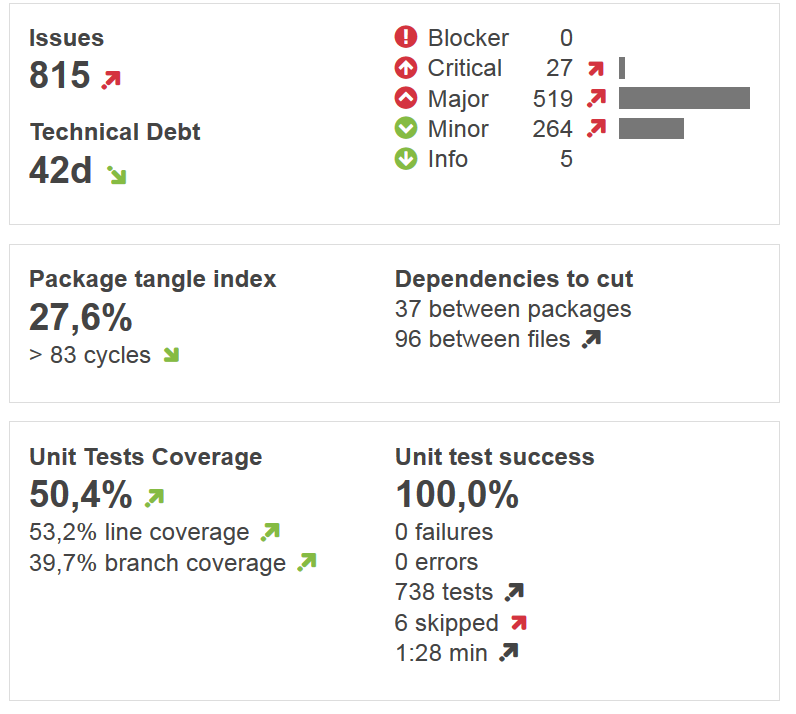
\includegraphics[scale=0.5]{statistics_group1}
	
\subsection*{Strategy}
\begin{itemize}
	\item Testing: Start with looking for a way to create an simple \emph{environment} to test the big classes like \emph{server} and \emph{client}. Also try to get PowerMock running (by waiting until it becomes compatible, or finding another method). Make sure to continue testing! 
	\item Issues \& Technical Debt: Issues are divided in Blocker, Critical, Major, Minor and Info. Make sure there are no Blocker and Critical issues and took at least look at the Major ones. This way you'll waste not to much time fixing issues compared to extending the code.  
	\item Decoupling: With \emph{Sonar} and \emph{Stan} you can visualize the dependencies. When you have an overview you can decide whether to change the class/package and try to cut dependencies. Sometimes restructuring will be needed. 
\end{itemize}
\subsection{Final words}
All in all, there are few things that the customer really wanted but we didn't implement because it was either too hard or simply impossible. Also, we were running short on time. The things that we didn't implement are the communication handicap (being able to communicate with another bot or not, or having a set chance that a certain message is going to be delivered) because this was too hard to do given the communication of GOAL-programmed agents, and the path finding and collisions of robots (robots can or cannot walk over each other in a path), because this was hard to do and we had time constraints. These are functionalities that can be added by new teams further developing the software.
\end{document}
